\section{The excitation condition: what a trajectory has to do}
\label{sec:excitation}
%==========================================================================

\emph{Everything so far says what a record confined to a band cannot deliver. This
section says what a record would have to do instead, and it is the link between the
obstruction and the data specification.}

\subsection{The parametrisation, pinned}
\label{sec:pinned}

Nothing below can be proved until one choice is made explicit, because the two natural
parametrisations give different statements. The enzymatic flux is written
\begin{equation}
\theta\, g(m), \qquad g(m) = \frac{m}{K_m+m},
\label{eq:pin}
\end{equation}
with $\theta$ \emph{absorbing} the maximal velocity: $\theta$ \emph{is} the patient's
residual $V_{\max}$, not a fraction of a population $V_{\max}$. Carrying the two
separately, as $V_{\max}\theta\, g(m)$ with $\theta \in [0,1]$, adds a parameter that no
excursion separates, since only the product multiplies $g$. Splitting them requires an
anchor outside the marker, and the $1$-$^{13}$C-propionate breath test is what such an
anchor looks like~\cite{breath_test_mma}. % C48
The dynamic model is then
\begin{equation}
\dot m \;=\; L(t) + L_0 \;-\; \bigl(\theta + \Delta(t)\bigr) g(m) \;-\; k_e\, m ,
\label{eq:dyn}
\end{equation}
with $L$ the recorded component of the propiogenic load, $L_0$ its unrecorded component
carried as an unknown constant, and $\Delta$ the therapeutic increment, known from the
dosing schedule.

\subsection{Both ends are degenerate, and they fail differently}

\begin{proposition}[Two degeneracies]
\label{prop:excitation}
In \eqref{eq:dyn} with $(\theta, K_m, k_e, L_0)$ unknown:
\begin{enumerate}[leftmargin=*, itemsep=2pt]
\item \textbf{Below the half-saturation level.} As $m/K_m \to 0$, $g(m) \to m/K_m$ and
total clearance collapses to $\left(\theta/K_m + k_e\right) m$. Three of the four
sensitivity directions become proportional to $m$, so only the lumped ratio
$\theta/K_m + k_e$ is identifiable and $\theta$, $K_m$ and $k_e$ are not separable.
\item \textbf{Above it.} As $m/K_m \to \infty$, $g(m) \to 1$ and \eqref{eq:dyn} becomes
$\dot m = L(t) + L_0 - \theta - k_e m$. \textbf{$\theta$ enters only through
$L_0 - \theta$}, so with $L_0$ unknown the residual capacity and the unrecorded load are
confounded and cannot be separated from the marker trajectory at all.
\end{enumerate}
\end{proposition}

\begin{proof}[Argument]
Both are limits of the sensitivity matrix. Writing the four columns as derivatives of the
ordinate with respect to $(\ln\theta, \ln K_m, \ln k_e, L_0)$,
\[
\Bigl(\theta g(m),\;\; -\theta K_m \tfrac{m}{(K_m+m)^2},\;\; k_e m, \;\; 1 \Bigr),
\]
the first three tend to $\bigl(\theta m/K_m,\, -\theta m/K_m,\, k_e m\bigr)$ as
$m/K_m \to 0$, all proportional to $m$ and hence of rank one together with the constant
fourth; and to $(\theta,\, 0,\, k_e m)$ as $m/K_m \to \infty$, where the first coincides
with the fourth. Rank two at both ends.
\end{proof}

\textbf{The two failures are not equally survivable.} At the low end a decomposition is
lost while the clearance itself stays constrained: the data still say what the patient
eliminates, they do not say through which channel. At the high end the target parameter is
lost against a quantity nobody records. The earlier phrasing of this note --- ``below $K_m$
only the lumped ratio, above $K_m$ only the product'' --- was wrong in the second clause,
and wrong in the direction that matters.

\begin{remark}[Which makes the load record load-bearing]
\label{rem:load_bearing}
Proposition~\ref{prop:excitation}(2) is conditional on $L_0$ being unknown. If the load
were recorded exactly, saturation would be the \emph{best} place to measure, not the worst:
$C(m) \to \theta + k_e m$ and the intercept of that line is $\theta$ outright, with no
extrapolation and no $K_m$. Figure~\ref{fig:D1}~(right) draws both cases, and they differ
qualitatively: with the load known, $\operatorname{sd}(\ln\hat\theta)$ falls monotonically
as the patient is carried up the curve; with it partly unrecorded, the optimum is
\emph{interior}.

So load-recording precision is not a mechanical detail to be tidied up at the end. It is
what creates the upper obstruction, and it is therefore the first thing on the data
specification of Section~\ref{sec:spec}.
\end{remark}

\subsection{Identifiability comes from curvature, and there is a closed form}

Since both ends are flat, what separates the parameters is the \emph{change} in the
saturation across the visited range. The ratio of the $K_m$ sensitivity to the $\theta$
sensitivity is
\begin{equation}
\frac{\partial C/\partial \ln K_m}{\partial C/\partial \ln \theta}
\;=\; -\bigl(1 - g(m)\bigr) \;=\; -\varphi(m),
\qquad \varphi(m) = \frac{K_m}{K_m + m},
\label{eq:phi}
\end{equation}
and the ratio of the $k_e$ sensitivity to it is $(k_e/\theta)(K_m + m)$, which is affine in
$m$ and which any excursion excites. It is $\varphi$ that is flat at both ends, so the
quantity a design has to buy is the drop in $\varphi$ across the band:
\begin{equation}
E \;=\; \varphi(m_{\min}) - \varphi(m_{\max})
\;=\; \frac{K_m\,(m_{\max} - m_{\min})}{(K_m + m_{\min})(K_m + m_{\max})} .
\label{eq:E}
\end{equation}

\begin{proposition}[The excitation is maximised straddling $K_m$]
\label{prop:straddle}
Fix the fold range $r = m_{\max}/m_{\min} > 1$. Then $E$ is maximised at
\begin{equation}
m_{\min} = \frac{K_m}{\sqrt r}, \qquad m_{\max} = K_m \sqrt r,
\qquad\text{that is}\qquad \sqrt{m_{\min} m_{\max}} = K_m ,
\label{eq:straddle}
\end{equation}
and there
\begin{equation}
E_{\max}(r) \;=\; \frac{\sqrt r - 1}{\sqrt r + 1},
\qquad\text{so a required $E$ needs}\qquad
r \;\ge\; \left(\frac{1+E}{1-E}\right)^{\!2} .
\label{eq:Emax}
\end{equation}
\end{proposition}

\begin{proof}
Put $x = m_{\min}/K_m$, so $E = (1+x)^{-1} - (1+rx)^{-1}$. Then
$\partial E/\partial x = -(1+x)^{-2} + r(1+rx)^{-2}$, which vanishes when
$\sqrt r\,(1+x) = 1 + rx$, that is at $x = 1/\sqrt r$. Substituting gives
$E_{\max} = \sqrt r/(\sqrt r + 1) - 1/(1 + \sqrt r)$, which is \eqref{eq:Emax}, and
inverting it gives the requirement on $r$.
\end{proof}

\textbf{The requirement is a band around $K_m$, not a threshold above it.} That is the
correction this section exists to make, and it changes what a protocol should ask for. A
band of a given fold range placed a decade below $K_m$ delivers a fraction of what the same
fold range delivers straddling it: at $r = 2$, the band the illustrative patient is held in
gives $E = 0.058$ against a possible $0.172$, a factor of three thrown away by placement
alone. Across four decades of operating point the penalty is far larger than that, because
$\operatorname{sd}(\ln\hat\theta)$ depends on placement more steeply than $E$ does:
\textbf{at the operating point this note's patient is managed to, it is about $2\,100$ times
its best} (Figure~\ref{fig:D1}).

\begin{figure}[htbp]
\centering
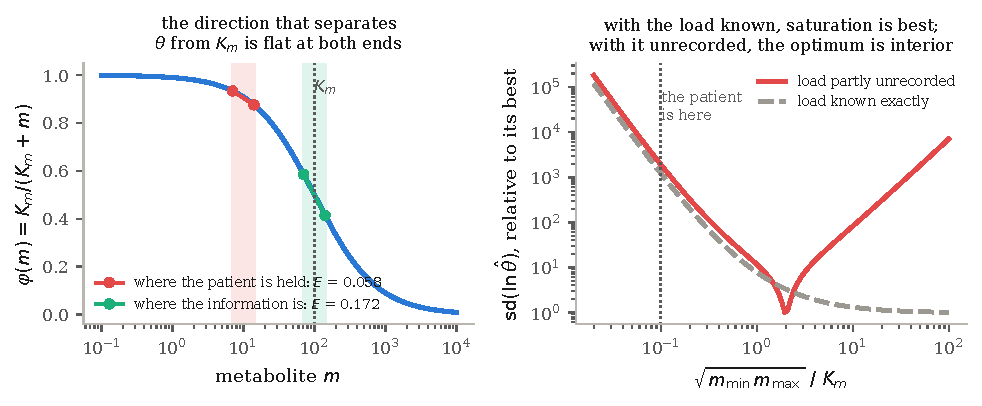
\includegraphics[width=\textwidth]{fig_D1_excitation.pdf}
\caption{The excitation condition. \textbf{Left:} $\varphi(m) = K_m/(K_m+m)$, the direction
that separates $\theta$ from $K_m$. It is flat at both ends of the saturation curve, so the
information a band carries is the \emph{drop} in $\varphi$ across it,
\eqref{eq:E}. The two shaded bands have the same fold range and differ only in where they
sit. \textbf{Right:} the price of sitting in the wrong place, as
$\operatorname{sd}(\ln\hat\theta)$ against the geometric centre of the band. With the load
known exactly the curve is monotone and saturation is the best place to measure; with the
load partly unrecorded the optimum is interior, because
Proposition~\ref{prop:excitation}(2) then bites. The dotted line is where clinical
management holds the patient.}
\label{fig:D1}
\end{figure}

\begin{remark}[Two ways to buy the same information, and only one of them is available]
\label{rem:two_buys}
Equation \eqref{eq:Emax} says a required excitation can be met either by a wide band
wherever the patient is, or by a narrow band placed correctly. The two are not
interchangeable clinically. Reaching the neighbourhood of $K_m$ means carrying the marker
to roughly twenty times its managed level, which is a decompensation; buying the same
information from the operating point instead needs a fold range of order ten, which is also
a decompensation, reached from below. \textbf{The safety constraint is on the level, and both
routes violate it.} What separates them is that the first is cheap in width and the second
is cheap in level, so a protocol that has any room at all should spend it on placement
rather than on duration.
\end{remark}

\vspace{0.5em}
\hrule
\vspace{1em}

%==========================================================================
